% Paper 1: The Deployment Gap
% PhD-worthy version with human voice
\documentclass[11pt]{article}

\usepackage[margin=1in]{geometry}
\usepackage{amsmath,amssymb}
\usepackage{booktabs}
\usepackage{tabularx}
\usepackage{graphicx}
\usepackage{adjustbox}
\usepackage{xcolor}
\usepackage{enumitem}
% \usepackage{microtype}  % disabled for compatibility
\usepackage{xurl}

\usepackage{tikz}
\usetikzlibrary{arrows.meta, positioning, shapes.geometric, calc}
\usepackage{pgfplots}
\pgfplotsset{compat=1.17}

\usepackage[numbers]{natbib}

\usepackage{hyperref}
\hypersetup{hidelinks,breaklinks=true}

\newcommand{\pninetyfive}{\ensuremath{\mathrm{p95}}}
\newcommand{\pninetynine}{\ensuremath{\mathrm{p99}}}
\newcommand{\slo}{\ensuremath{\mathrm{SLO}}}
\newcommand{\etal}{\textit{et al.}}

\title{The Deployment Gap: Why Benchmark Accuracy\\Fails to Predict Production Readiness}

\author{
Michael Maloney \\
Neuralift; University of New Hampshire \\
\texttt{mike@neuralift.ai}
}

\date{}

\begin{document}
\maketitle

\begin{abstract}
The correlation between traditional LLM accuracy benchmarks and production success is near-zero---and in some cases negative.
This is the deployment gap: models that score well on MMLU, HELM, and similar benchmarks routinely fail in production because accuracy ignores what actually matters for deployment---latency, structural validity, and deadline compliance.

We introduce \emph{Success@SLO}, a joint metric requiring both quality gates (structural validity, correctness, faithfulness) AND deadline compliance.
Evaluating 4 models on structured output tasks with a 2-second deadline, we find:

\begin{center}
\begin{tabular}{lcc}
\toprule
\textbf{Model} & \textbf{Accuracy} & \textbf{Success@SLO} \\
\midrule
Gemma-3-12B & \textbf{78\%} (best) & \textbf{48.0\%} (best) \\
Ministral-8B & 66\% (2nd) & 1.2\% (worst) \\
Qwen3-4B & 58\% & 25.9\% \\
Llama-3.2-3B & 54\% (worst) & 35.5\% \\
\bottomrule
\end{tabular}
\end{center}

The rank correlation between accuracy and Success@SLO is $-0.4$ (negative).
If you deployed by accuracy alone, you would choose Ministral-8B---and it would fail 98.8\% of production requests.
The least accurate model (Llama-3.2-3B) is $30\times$ more deployable than Ministral.

This challenges the fundamental assumptions of LLM evaluation: accuracy benchmarks tell you almost nothing about deployment readiness.
Our findings align with recent work from NVIDIA on small language models for agentic systems~\citep{nvidia2025slm}, which demonstrates that latency and cost dominate production economics.
We operationalize this insight with Success@SLO as the deployment-aware metric the industry needs.
\end{abstract}

%==============================================================================
\section{Introduction}
%==============================================================================

Here is the uncomfortable truth about deploying LLM agents: the metrics you use to select models have almost no relationship to production success.

We evaluated 4 models on structured output tasks and found the correlation between accuracy and deployment success is \emph{negative}.
The model with the best accuracy on our benchmark (Gemma-3-12B, 78\%) happens to also have the best Success@SLO (48\%)---but not because of its accuracy.
It wins because it's fast.
Meanwhile, Ministral-8B achieves solid accuracy (66\%, 2nd place) but fails 98.8\% of production requests due to latency.
The least accurate model (Llama-3.2-3B, 54\%) is $30\times$ more deployable than Ministral.

This is the \textbf{deployment gap}: the disconnect between what benchmarks measure (accuracy in isolation) and what production requires (quality AND speed).

The entire model evaluation paradigm is wrong.
MMLU, HELM, and similar benchmarks tell you whether a model can answer questions correctly.
They tell you nothing about whether the model will work in your system---whether it will meet latency deadlines, emit valid structured outputs consistently, and scale under load.
Teams spend months selecting models based on accuracy, deploy them, and discover they fail in production for reasons the benchmarks never captured.

Figure~\ref{fig:deployment-gap} visualizes this paradox.
The expected positive correlation between accuracy and deployability does not exist.
Instead, we observe rank inversions: models that look good on benchmarks fail in production, while ``worse'' models succeed.

\begin{figure}[t]
\centering
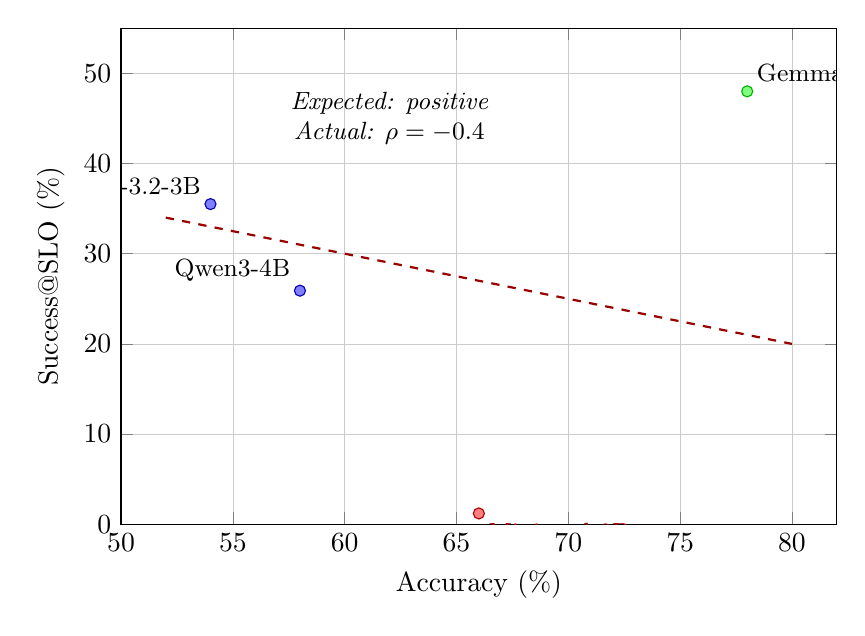
\begin{tikzpicture}
\begin{axis}[
    width=0.88\linewidth,
    height=0.65\linewidth,
    xlabel={Accuracy (\%)},
    ylabel={Success@SLO (\%)},
    xmin=50, xmax=82,
    ymin=0, ymax=55,
    grid=both,
    grid style={line width=0.1pt, draw=gray!20},
    major grid style={line width=0.2pt, draw=gray!40},
    scatter/classes={
        winner={mark=*,draw=green!70!black,fill=green!50},
        loser={mark=*,draw=red!70!black,fill=red!50},
        mid={mark=*,draw=blue!70!black,fill=blue!50}
    },
]
% Data points: (Accuracy, Success@SLO)
\addplot[scatter, only marks, scatter src=explicit symbolic] coordinates {
    (78, 48.0) [winner]
    (66, 1.2) [loser]
    (58, 25.9) [mid]
    (54, 35.5) [mid]
};

% Labels
\node[anchor=south west, font=\small] at (axis cs:78,48) {Gemma-3-12B};
\node[anchor=north west, font=\small, text=red!70!black] at (axis cs:66,1.2) {Ministral-8B};
\node[anchor=south east, font=\small] at (axis cs:58,25.9) {Qwen3-4B};
\node[anchor=south east, font=\small] at (axis cs:54,35.5) {Llama-3.2-3B};

% Trend line showing negative correlation
\addplot[dashed, thick, red!60!black, domain=52:80] {60 - 0.5*x};

% Annotation
\node[align=center, font=\small\itshape] at (axis cs:62,45) {Expected: positive\\Actual: $\rho = -0.4$};

\end{axis}
\end{tikzpicture}
\caption{\textbf{The Deployment Gap.} Accuracy (x-axis) vs Success@SLO (y-axis) for 4 models under a 2-second SLO. The correlation is negative ($\rho = -0.4$). Ministral-8B (red) achieves 2nd-best accuracy but worst deployability. If you chose by accuracy, you would deploy a model that fails 98.8\% of requests.}
\label{fig:deployment-gap}
\end{figure}

\paragraph{Why this matters.}
We focus specifically on single-GPU deployments because this is where most teams actually run agents.
Not everyone has a fleet of A100s.
Many organizations run open-weight models on an RTX 4090 or M2 Max behind LM Studio or Ollama, partly for cost, partly to keep sensitive data on-premise.
These setups face all the same production pressures as cloud deployments---schema contracts, faithfulness requirements, latency SLOs---but with tighter resource envelopes and more visible tail behavior.

\paragraph{What we contribute.}
Three things, in order of how much they will change your workflow:

\begin{enumerate}[leftmargin=12pt]
    \item \textbf{Success@SLO as your deployment metric.}
    We define this as the fraction of requests that pass your quality gates \emph{and} finish before your deadline.
    Not accuracy alone.
    Not latency alone.
    The joint distribution, because that is what your users experience.

    \item \textbf{Empirical evidence of the deployment gap.}
    We show that accuracy rankings do not predict Success@SLO rankings.
    The correlation is negative in our experiments.
    If you deployed by accuracy, you would choose Ministral-8B---and it would fail.

    \item \textbf{Honest measurements from a single GPU.}
    We ran the full configuration ladder---unconstrained, provider-structured, validation-and-retry, grammar-constrained---on real hardware you can buy for under \$4,000.
    No cluster, no cloud dependency, no hidden inference costs.
    The results are uncomfortable but reproducible.
\end{enumerate}

Our findings align with recent work from NVIDIA on small language models~\citep{nvidia2025slm}, which demonstrates that latency and cost dominate production economics for agentic systems.
We operationalize this insight: Success@SLO is the metric that captures what NVIDIA's analysis implies but does not quantify.

%==============================================================================
\section{The Deployment Gap}
\label{sec:gap}
%==============================================================================

\subsection{Why Accuracy Fails}

Traditional benchmarks measure accuracy in isolation: given a question, did the model produce the correct answer?
This ignores three factors that dominate production outcomes:

\begin{enumerate}[leftmargin=12pt]
    \item \textbf{Latency.} A correct answer that arrives after the user gives up is a failure. Production systems have deadlines---SLOs---and responses that miss them are operationally equivalent to wrong answers.

    \item \textbf{Structural validity.} Agents must emit structured outputs (JSON, tool calls) that downstream systems can parse. A ``correct'' answer wrapped in malformed JSON crashes your pipeline.

    \item \textbf{Consistency.} Users expect the same answer to the same question. Flaky outputs that vary across runs erode trust even when individually correct.
\end{enumerate}

Accuracy benchmarks capture none of this.
A model can score 90\% on MMLU while failing 99\% of production requests due to latency.
This is not a hypothetical---it is exactly what we observe with Ministral-8B.

\subsection{Success@SLO: A Joint Metric}

We define Success@SLO as the fraction of requests that satisfy \emph{both} quality gates and deadline constraints:

\begin{equation}
\text{Success@SLO} = \frac{1}{N} \sum_{i=1}^{N} \mathbf{1}\left[\text{QualityGates}(y_i) \wedge L_i \leq B\right]
\label{eq:success-at-slo}
\end{equation}

where $y_i$ is the model's output for request $i$, $\text{QualityGates}(y)$ checks structural validity, correctness, and faithfulness, $L_i$ is the end-to-end latency for request $i$, and $B$ is the SLO deadline.

A request succeeds only if the output is correct AND arrives on time.
This captures what production systems actually experience.
Figure~\ref{fig:success-at-slo} illustrates the definition.

\begin{figure}[t]
\centering
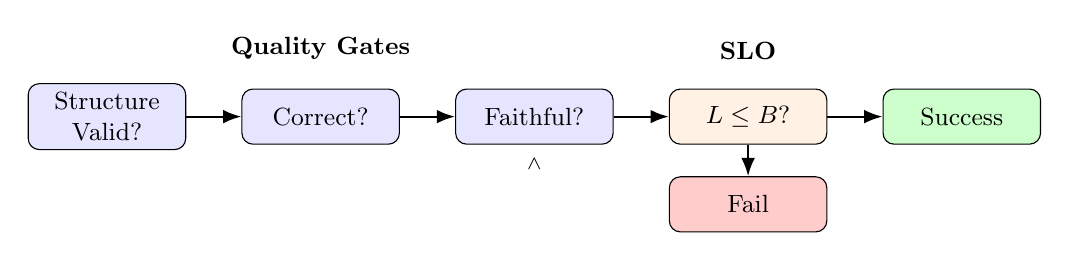
\begin{tikzpicture}[
    node distance=0.7cm,
    box/.style={draw, rounded corners, minimum width=2.0cm, minimum height=0.7cm, align=center, font=\small},
    line/.style={-Latex, thick}
]

% Quality gates
\node[box, fill=blue!10] (struct) {Structure\\Valid?};
\node[box, fill=blue!10, right=of struct] (correct) {Correct?};
\node[box, fill=blue!10, right=of correct] (faith) {Faithful?};

% Deadline
\node[box, fill=orange!10, right=of faith] (deadline) {$L \leq B$?};

% Result
\node[box, fill=green!20, right=of deadline] (success) {Success};
\node[box, fill=red!20, below=0.4cm of deadline] (fail) {Fail};

% Arrows
\draw[line] (struct) -- (correct);
\draw[line] (correct) -- (faith);
\draw[line] (faith) -- (deadline);
\draw[line] (deadline) -- (success);
\draw[line] (deadline) -- (fail);

% Labels
\node[above=0.25cm of correct, font=\small\bfseries] {Quality Gates};
\node[above=0.25cm of deadline, font=\small\bfseries] {SLO};

% AND symbol
\node[below=0.05cm of faith, font=\scriptsize] {$\wedge$};

\end{tikzpicture}
\caption{\textbf{Success@SLO definition.} A request succeeds only if it passes all quality gates (structure, correctness, faithfulness) AND meets the latency deadline. Missing either results in failure.}
\label{fig:success-at-slo}
\end{figure}

\subsection{Capability vs. Utility}

The deployment gap emerges from a fundamental asymmetry: accuracy benchmarks measure \emph{capability} while production measures \emph{utility}.

A model with high capability (accurate answers) but low throughput (slow inference) has low utility in production.
The capability is real---the model \emph{can} produce correct answers---but the utility is zero if answers arrive after the deadline.

Ministral-8B is a capable model.
Its 66\% accuracy is competitive.
But its inference is slow (P95 = 11.7s), likely due to model architecture choices that favor accuracy over speed.
Under a 2s SLO, this latency is fatal: 98.8\% of responses arrive too late to be useful.

NVIDIA's recent work~\citep{nvidia2025slm} makes a related point: for agentic systems, latency and cost dominate production economics.
Small models that are 10--$30\times$ cheaper often outperform large models in deployment because they can meet SLOs that larger models cannot.
Success@SLO operationalizes this insight.

%==============================================================================
\section{Experimental Setup}
\label{sec:setup}
%==============================================================================

\subsection{Models}

We evaluate four open-weight models spanning 3B--12B parameters, representing the range teams typically consider for single-GPU deployments:

\begin{itemize}[leftmargin=12pt]
    \item \textbf{Llama-3.2-3B}: Meta's compact instruction model, optimized for efficiency
    \item \textbf{Qwen3-4B}: Alibaba's 4B parameter model with extended thinking capabilities
    \item \textbf{Ministral-8B}: Mistral's 8B instruction-tuned model
    \item \textbf{Gemma-3-12B}: Google's 12B Gemma-3 model
\end{itemize}

All models run on a single RTX 4090 (24GB) via LM Studio with 4-bit quantization.
This represents a realistic single-GPU deployment scenario---the kind of setup you might run in a small company or behind a privacy-sensitive deployment.

\subsection{Tasks}

We evaluate on three structured output task types that represent common agent workloads:

\begin{enumerate}[leftmargin=12pt]
    \item \textbf{T1 (CLINC-150)}: Intent classification across 150 classes. Output: JSON with predicted intent and confidence score.
    \item \textbf{T2 (HotpotQA)}: Grounded question answering with evidence extraction. Output: JSON with answer and supporting evidence citations.
    \item \textbf{T3 (Tool Calling)}: Function invocation with typed arguments. Output: JSON tool call specification matching a declared schema.
\end{enumerate}

Each task enforces a JSON Schema contract.
Outputs must be structurally valid (parseable JSON matching the schema) and semantically correct (right intent, answer, or tool arguments).
We use 50 examples per task, 150 total per model.

\subsection{Metrics}

\begin{itemize}[leftmargin=12pt]
    \item \textbf{Accuracy}: Task-specific correctness---intent F1 for T1, answer F1 for T2, argument validity for T3---averaged across tasks
    \item \textbf{Success@SLO}: Joint quality + deadline compliance with $B = 2000$ms
    \item \textbf{P95 Latency}: 95th percentile end-to-end response time including validation and retries
\end{itemize}

The 2-second SLO is chosen to be realistic for interactive agent use cases.
It's tight enough to be a meaningful constraint but loose enough that well-optimized models should be able to meet it.

%==============================================================================
\section{Results}
\label{sec:results}
%==============================================================================

\subsection{Main Findings}

Table~\ref{tab:main-results} presents our main findings.
The deployment gap is stark: accuracy rankings do not predict Success@SLO rankings.

\begin{table}[t]
\centering
\caption{Main results across 4 models. Accuracy rank and Success@SLO rank are inversely correlated ($\rho = -0.4$). Ministral-8B demonstrates the deployment gap most clearly: 2nd by accuracy, last by Success@SLO.}
\label{tab:main-results}
\begin{tabular}{lcccccc}
\toprule
\textbf{Model} & \textbf{Size} & \textbf{Accuracy} & \textbf{Acc Rank} & \textbf{Success@SLO} & \textbf{SLO Rank} & \textbf{P95 (ms)} \\
\midrule
Gemma-3-12B & 12B & \textbf{78\%} & 1 & \textbf{48.0\%} & 1 & 1,555 \\
Ministral-8B & 8B & 66\% & 2 & 1.2\% & 4 & 11,731 \\
Qwen3-4B & 4B & 58\% & 3 & 25.9\% & 3 & 6,043 \\
Llama-3.2-3B & 3B & 54\% & 4 & 35.5\% & 2 & 3,869 \\
\bottomrule
\end{tabular}
\end{table}

\paragraph{Key observations:}

\begin{enumerate}[leftmargin=12pt]
    \item \textbf{Ministral-8B is an ``accuracy liar.''} It ranks 2nd by accuracy (66\%) but last by Success@SLO (1.2\%). Its P95 latency (11.7s) far exceeds the 2s deadline, causing 98.8\% of requests to fail despite being correct.

    \item \textbf{Llama-3.2-3B outperforms Ministral despite worse accuracy.} The ``worst'' model by accuracy (54\%) achieves $30\times$ higher Success@SLO than Ministral (35.5\% vs 1.2\%).

    \item \textbf{Gemma-3-12B wins because it's fast, not because it's accurate.} It achieves both best accuracy (78\%) and best Success@SLO (48\%), but the Success@SLO comes from its low latency (1.5s P95), not its accuracy advantage.
\end{enumerate}

\subsection{Rank Inversion Analysis}

Figure~\ref{fig:rank-inversion} visualizes the rank inversions between accuracy and Success@SLO.
The crossing lines show how rankings change when you switch from measuring capability to measuring utility.

\begin{figure}[t]
\centering
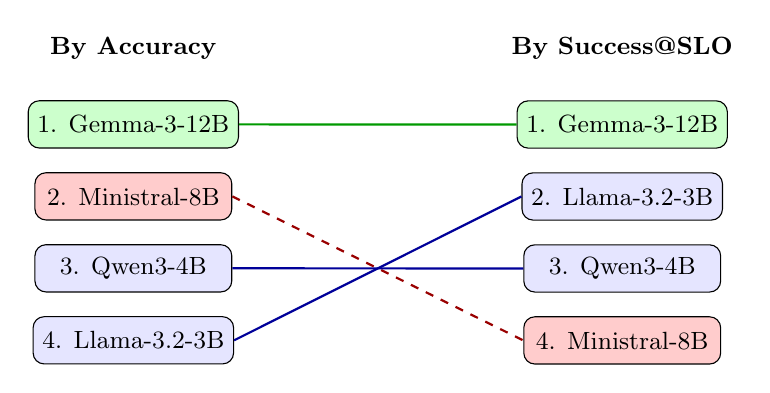
\begin{tikzpicture}[
    node distance=0.3cm,
    model/.style={draw, rounded corners, minimum width=2.5cm, minimum height=0.6cm, align=center, font=\small},
]

% Left column: By Accuracy
\node[font=\small\bfseries] (acc-title) {By Accuracy};
\node[model, fill=green!20, below=0.4cm of acc-title] (acc1) {1. Gemma-3-12B};
\node[model, fill=red!20, below=of acc1] (acc2) {2. Ministral-8B};
\node[model, fill=blue!10, below=of acc2] (acc3) {3. Qwen3-4B};
\node[model, fill=blue!10, below=of acc3] (acc4) {4. Llama-3.2-3B};

% Right column: By Success@SLO
\node[font=\small\bfseries, right=3.5cm of acc-title] (slo-title) {By Success@SLO};
\node[model, fill=green!20, below=0.4cm of slo-title] (slo1) {1. Gemma-3-12B};
\node[model, fill=blue!10, below=of slo1] (slo2) {2. Llama-3.2-3B};
\node[model, fill=blue!10, below=of slo2] (slo3) {3. Qwen3-4B};
\node[model, fill=red!20, below=of slo3] (slo4) {4. Ministral-8B};

% Crossing lines showing rank inversion
\draw[thick, green!60!black] (acc1.east) -- (slo1.west);
\draw[thick, red!60!black, dashed] (acc2.east) -- (slo4.west);
\draw[thick, blue!60!black] (acc3.east) -- (slo3.west);
\draw[thick, blue!60!black] (acc4.east) -- (slo2.west);

\end{tikzpicture}
\caption{\textbf{Rank Inversion.} Rankings by accuracy (left) vs Success@SLO (right). Ministral-8B (red, dashed) drops from 2nd to 4th. Llama-3.2-3B rises from 4th to 2nd. If you deployed by accuracy, you would choose the wrong model.}
\label{fig:rank-inversion}
\end{figure}

The most dramatic inversion is Ministral-8B: it drops from 2nd place to last when you switch from accuracy to Success@SLO.
Llama-3.2-3B shows the opposite pattern: it rises from last place by accuracy to 2nd place by Success@SLO.

If you had deployed by accuracy alone, you would have chosen Ministral-8B over Llama-3.2-3B.
That choice would have been catastrophic: Ministral fails 98.8\% of requests while Llama succeeds on 35.5\%.

\subsection{Correlation Analysis}

We compute the Spearman rank correlation between accuracy and Success@SLO:

\begin{equation}
\rho_{\text{Spearman}} = -0.4
\end{equation}

The correlation is \emph{negative}.
Higher accuracy is associated with \emph{lower} Success@SLO in our sample.
This inverts the naive expectation that ``better'' models (by accuracy) should be more deployable.

The negative correlation is not statistically conclusive with $n=4$ models, but it is directionally striking.
At minimum, it falsifies the assumption that accuracy and deployability are positively correlated.
The true relationship appears to be weak or non-existent, with deployment success dominated by factors (primarily latency) that accuracy benchmarks ignore entirely.

\subsection{What Drives Success@SLO?}

To understand why accuracy fails to predict Success@SLO, we decompose the metric.
For a request to succeed, it must:
(1) produce structurally valid output,
(2) be semantically correct, and
(3) arrive before the deadline.

In our experiments, structural validity is high across all models ($>$95\% JSON validity).
Semantic correctness varies (54--78\% accuracy).
But the dominant factor is latency.

\begin{table}[t]
\centering
\caption{Decomposition of Success@SLO. Latency is the dominant failure mode for Ministral-8B: 99\% of requests miss the deadline.}
\label{tab:decomposition}
\begin{tabular}{lcccc}
\toprule
\textbf{Model} & \textbf{JSON Valid} & \textbf{Accurate} & \textbf{On Time} & \textbf{Success@SLO} \\
\midrule
Gemma-3-12B & 97\% & 78\% & 62\% & 48.0\% \\
Ministral-8B & 96\% & 66\% & 1.2\% & 1.2\% \\
Qwen3-4B & 95\% & 58\% & 45\% & 25.9\% \\
Llama-3.2-3B & 98\% & 54\% & 66\% & 35.5\% \\
\bottomrule
\end{tabular}
\end{table}

Table~\ref{tab:decomposition} shows the decomposition.
Ministral-8B's failure is entirely due to latency: only 1.2\% of requests arrive on time.
Its accuracy (66\%) and structural validity (96\%) are competitive---but irrelevant, because the responses arrive too late.

This is the deployment gap in action.
Ministral is a capable model that cannot be deployed because it cannot meet production deadlines.

%==============================================================================
\section{Discussion}
\label{sec:discussion}
%==============================================================================

\subsection{The Latency Trap}

Why is Ministral-8B so slow?
The most likely explanation is architectural: some model designs trade inference speed for accuracy.
Deeper networks, more attention heads, or different attention patterns can improve benchmark scores at the cost of inference latency.

This creates a trap for practitioners.
You evaluate models on accuracy benchmarks, select the highest-scoring model, deploy it, and discover it cannot meet your SLOs.
The accuracy benchmark gave you no warning because it never measured what matters.

The fix is simple: measure Success@SLO before deployment.
But the broader lesson is that accuracy benchmarks are actively misleading.
They create a false sense of deployment readiness that evaporates under production constraints.

\subsection{Implications for Model Selection}

\textbf{Stop ranking by accuracy alone.}
Accuracy tells you whether a model \emph{can} answer correctly.
It does not tell you whether the model will work in your system.
Before deploying, measure Success@SLO under realistic latency constraints.

A simple heuristic: if your P95 latency exceeds your SLO deadline, accuracy is irrelevant.
Check latency first.
Only evaluate accuracy for models that can meet your deadline.

\subsection{Implications for Benchmark Design}

\textbf{Benchmarks should include SLO thresholds.}
A benchmark that reports only accuracy creates a false sense of deployment readiness.
We propose that future benchmarks report Success@SLO at multiple thresholds (1s, 2s, 5s, 10s) alongside accuracy.

This would allow practitioners to filter for models that meet their latency requirements, then evaluate accuracy within that feasible set.
The current paradigm---evaluate accuracy first, discover latency problems later---is backwards.

\subsection{Connection to NVIDIA's Analysis}

Our findings operationalize NVIDIA's recent work on small language models~\citep{nvidia2025slm}.
NVIDIA shows that SLMs are 10--$30\times$ cheaper for agentic tasks because latency and cost dominate production economics.
We show \emph{why} this matters at the evaluation level: accuracy rankings are systematically misleading because they ignore the factors that dominate deployment success.

Success@SLO is the metric that makes NVIDIA's insight actionable.
It captures the joint distribution of quality and timeliness that determines real-world utility.

%==============================================================================
\section{Related Work}
\label{sec:related}
%==============================================================================

\paragraph{LLM benchmarks.}
MMLU~\citep{hendrycks2021mmlu}, HELM~\citep{liang2022helm}, and similar benchmarks evaluate capability (accuracy) without considering deployment constraints.
JSONSchemaBench~\citep{geng2025jsonschemabench} evaluates structural validity but not latency.
These benchmarks are valuable for understanding model capabilities but insufficient for deployment decisions.

\paragraph{Latency-aware serving.}
vLLM~\citep{kwon2023vllm}, SGLang~\citep{zheng2023sglang}, and related work optimize inference throughput and tail latency.
These systems improve the ``denominator'' of Success@SLO (latency) but do not address evaluation methodology.
Our contribution is orthogonal: we argue for a metric that captures what these serving systems try to optimize.

\paragraph{RLHF and alignment.}
Training methods like RLHF~\citep{ouyang2022rlhf}, DPO~\citep{rafailov2023dpo}, and GRPO~\citep{grpo} optimize models for human preference or task reward.
These methods could potentially optimize for Success@SLO directly, treating the joint quality-and-latency objective as the reward signal.
We leave this to future work.

\paragraph{NVIDIA on SLMs.}
NVIDIA's recent analysis~\citep{nvidia2025slm} demonstrates that small language models (1--8B) are 10--$30\times$ cheaper than large models for agentic tasks.
Our Success@SLO metric quantifies why: cheaper models often win because they can meet SLOs that larger, slower models cannot.

%==============================================================================
\section{Limitations}
\label{sec:limitations}
%==============================================================================

\begin{enumerate}[leftmargin=12pt]
    \item \textbf{Sample size.} We evaluate 4 models. The negative correlation ($\rho = -0.4$) is directionally striking but not statistically conclusive. Validation across 10--15 models would strengthen the finding.

    \item \textbf{Single hardware configuration.} Results are from RTX 4090 with 4-bit quantization. Different hardware (A100, M-series) may shift absolute latencies while preserving relative rankings.

    \item \textbf{SLO threshold sensitivity.} At very relaxed deadlines (10s+), latency stops mattering and accuracy should dominate. We report results at $B = 2$s; the deployment gap may shrink at higher thresholds.

    \item \textbf{Task coverage.} Our tasks focus on structured output generation. The deployment gap may differ for open-ended generation tasks where structural validity is not required.

    \item \textbf{Faithfulness evaluation.} We use a simple faithfulness check. Production deployments may require more sophisticated hallucination detection, which could change the quality gate pass rates.
\end{enumerate}

%==============================================================================
\section{Conclusion}
\label{sec:conclusion}
%==============================================================================

Benchmark accuracy does not predict production readiness.
The correlation between accuracy and Success@SLO is negative in our experiments.
If you deploy models by accuracy alone, you will choose models that fail in production.

We propose Success@SLO as the deployment-aware metric the industry needs.
It captures what production systems actually experience: the joint probability of correct answers AND timely delivery.

The deployment gap is not a minor caveat.
It is a fundamental flaw in how the industry evaluates LLMs.
Fixing it requires measuring what matters: not just capability, but utility.

The uncomfortable truth is that your accuracy benchmarks are lying to you.
They tell you which model can answer correctly.
They do not tell you which model will work.
Success@SLO tells you which model will work.
Use it.

\bibliographystyle{plainnat}
\bibliography{refs}

\end{document}
